\section{Implementing the framework as an extension of the RTOS \label{sec:extension}}

For this second approach, the idea comes from our discussions with the communities.
Instead of building the framework inside the kernel, we would implement the framework as a RTOS extension.
The extension would provide calls that would be used in the user space of the application.
This approach is later mentionned as the extension approach.

\subsection{Definition of RTOS extension}

Many RTOS allow developers to create their own extensions that will be used by other developers to enhance and add functionalities to their applications.
In these extensions, we can find libraries that integrates FTP, COAP or even a Shell.
To use those extensions, the developer needs to specify them in the \texttt{Makefile}.
Those libraries are called 'apps' for Contiki and 'modules' for RIOT.

\begin{minipage}{.45\textwidth}
\begin{lstlisting}[style=CStyle, language=make, caption=example of Makefile using the app \texttt{shell} with Contiki]
CONTIKI_PROJECT = example
all: $(CONTIKI_PROJECT)
CONTIKI = ../contiki

# Using the shell app
APPS += shell 

include $(CONTIKI)/Makefile.include
\end{lstlisting}
\end{minipage}\hfill
\begin{minipage}{.45\textwidth}
\begin{lstlisting}[style=CStyle, language=make, caption=example of Makefile using the module \texttt{shell} with RIOT]
APPLICATION = example
BOARD ?= native
RIOTBASE ?= $(CURDIR)/../riot

# Using the shell module
USEMODULE += shell 

include $(RIOTBASE)/Makefile.include
\end{lstlisting}
\end{minipage}

\subsection{Framework utilization}

The idea of this second approach is to be able to measure the context switching time without impacting the application.
With this in mind, we will make sure that our framework is called only two times per task iteration.
From these calls, we can deduce the context switching time.
The figure \ref{fig:internal-framework-ping} shows an example with two tasks.
The first task starts at the step A and ends at the step A'.
The context switch occurs between the step A' and the step B, this latter step being the start of the second task.
The step B' is the end of the second task.
The idea is to call the framework at each step, A, A', B and B', providing a unique ID.
The context switching time is measured between the step A' and B.
The next sections describe the implementation of this framework and how it is used with our simple application.

\begin{figure}[!ht]
  \centering
  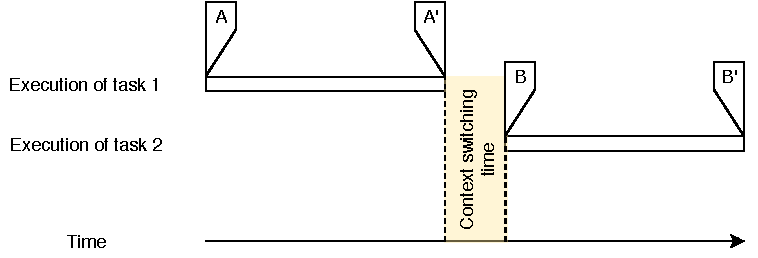
\includegraphics[scale=1]{assets/internal-framework-ping.pdf}
  \caption{\label{fig:internal-framework-ping}pings to the framework}
\end{figure}

\subsection{Using the framework with our simple application}

To understand the implementation of the framework, we need to understand what happens when our simple application boots. 
Then, we explain the implementation of the framework in the next section.

In the startup of our application, the first task is launched.
It will call the method \texttt{bench\_ping(TASK\_1)} where \texttt{TASK\_1} is the ID of the first task.
At this point, we enter in the framework space like shown in the figure \ref{fig:extension-activity-framework}.
The framework will check if the received ID from the \texttt{bench\_ping()} call is already stored in its context.
If the received ID match the one stored in the context or if no ID is stored in the context, no context switch occcured and the framework will reset its internal timer.
It also stores the received ID in its context.
The stored ID is now \texttt{TASK\_1}.
Once the first task ends its iteration and let the other task run, it calls the same method \texttt{bench\_ping(TASK\_1)} with its ID.
Once again, the framework checks the received ID and no change is detected.
It resets its internal timer.
The stored ID is still \texttt{TASK\_1}.

Now, the second task starts and call the framework with \texttt{bench\_ping(TASK\_2)} where \texttt{TASK\_2} is the ID of the second task.
The framework will detect an ID change by comparing the received ID, \texttt{TASK\_2}, with the stored ID in its context, \texttt{TASK\_1}.
This change means that a context switch occured.
We are between the step A' and B in the figure \ref{fig:internal-framework-ping}.
The framework will measure the context switching time by computing the difference between the actual timer and its internal timer.
The measure is then written on the serial port to be read by an external source like a computer.
The framework resets once again its timer and store the \texttt{TASK\_2} ID in its context.
In this way, we have computed the context switching time between the first and the second task.

\begin{figure}[!ht]
  \centering
  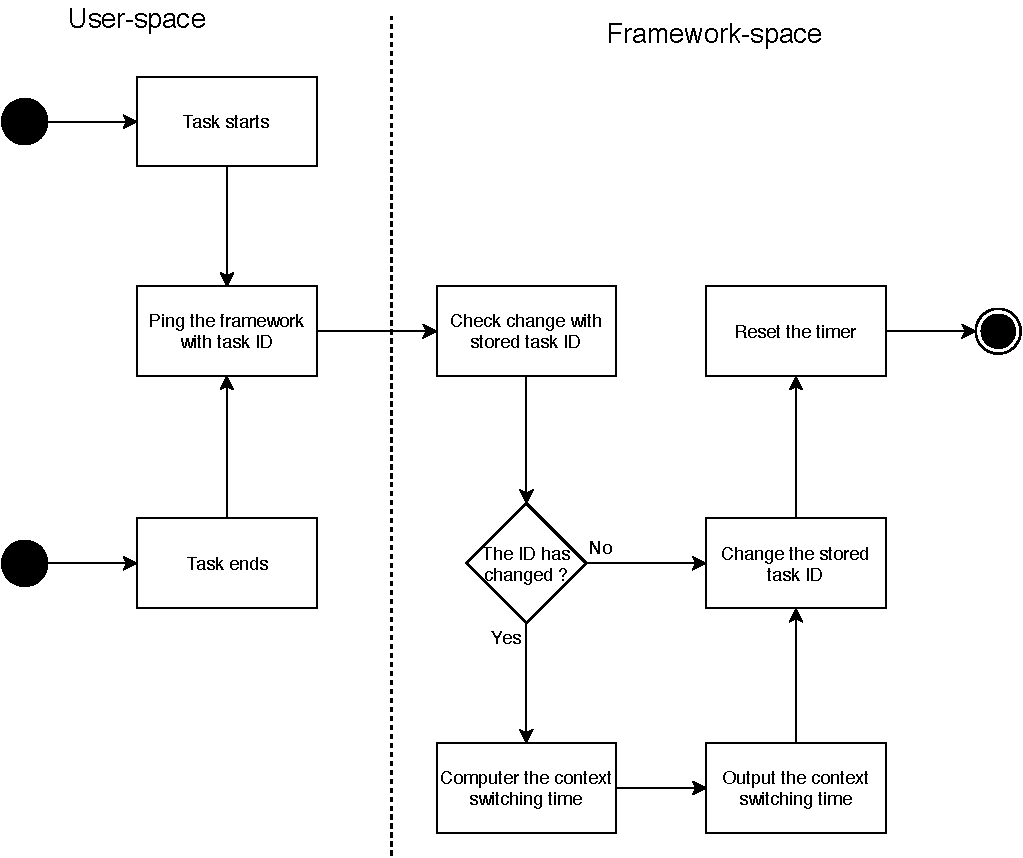
\includegraphics[scale=0.7]{assets/extension-activity-framework.pdf}
  \caption{activity flow of the framework\label{fig:extension-activity-framework}}
\end{figure}

\subsection{Framework implementation}

\subsubsection{Application source code}
For our simple application source code, we just added the call \texttt{bench\_ping()} at the start and the end of each task.
The listing \ref{lst:bench-task-code} shows how the task source code is impacted in Contiki.

\begin{lstlisting}[float, style=CStyle, label={lst:bench-task-code}, caption={source code of the application task with \texttt{bench\_ping()} calls}]
PROCESS_THREAD(task, ev, data)
{
    PROCESS_BEGIN();

    while (1)
    {
      bench_ping(TASK_ID); // Ping the framework
      // Wait for 1ms
      clock_delay_usec(1000);
      bench_ping(TASK_ID); // Ping the framework
      PROCESS_PAUSE();
    }

    PROCESS_END();
}
\end{lstlisting}

\subsubsection{Framework source code}

For the framework context, we store the received ID in the \texttt{new\_id} variable 
  and then use the \texttt{previous\_id} variable to check if a context switch occured.
The \texttt{current\_time} variable is the interval timer.
The code of the framework context is shown in the listing \ref{lst:context-code}.

\begin{lstlisting}[style=CStyle, float, label={lst:context-code}, caption={framework context implementation}]
struct BContext {
  uint32_t previous_id;
  uint32_t new_id;
  clock_time_t current_time;
} bench_context;
\end{lstlisting}

The \texttt{bench\_ping()} method will just saved the received ID in the \texttt{new\_id} variable 
  and then check if a change is detected like shown in the listing \ref{lst:bench-ping-code}.

\begin{lstlisting}[style=CStyle, float, label={lst:bench-ping-code}, caption={\texttt{bench\_ping()} implementation}]
void bench_ping(uint32_t id)
{
  bench_context.new_id = id;
  if (!check_change())
  {
    bench_context.current_time = RTIMER_NOW();
  }
}
\end{lstlisting}

When a change is detected, the framework will compute the context switching time 
  by retrieving the current time and computing its difference with the \texttt{current\_time} variable.
The time is computed in ticks for a better precision.
To retrieve the time in ticks, we used \texttt{RTIMER\_NOW()} in Contiki and \texttt{xtimer\_now().ticks32} in RIOT.
The internal timer is then reset just before writing the measure into the serial port.
Then the measure is written to the serial port using the \texttt{printf()} call.
The code of this measurement is shown in the listing \ref{lst:measurement-code}.

\begin{lstlisting}[style=CStyle, float, label={lst:measurement-code}, caption={source code of the benchmarking framework implemented in Contiki}]
// Compute the difference
clock_time_t previous = bench_context.current_time;
clock_time_t current = RTIMER_NOW();
clock_time_t result = current - previous;

// Keep the previous id for log
uint32_t previous_id = bench_context.previous_id;
// Change previous_id to new_id
bench_context.previous_id = bench_context.new_id;

bench_context.current_time = RTIMER_NOW(); // Ticks

printf("[BENCH_CONTEXT_SWITCHING] %lu %lu %lu\n", previous_id, bench_context.new_id, result);
\end{lstlisting}

All the source codes can be found in the Github repository\footnote{\url{https://github.com/bench-os/bench-os}}.